\documentclass[a4paper]{scrartcl}
\usepackage{drehbuch}
\usepackage{pdfpages}

\title{Modul - Vokabeltrainer}
\author{Hauke Schade\\Alexander Gräfenstein}
\date{\today}


%\modulhauptseite{Modultitel}
\newcommand{\modulhauptseite}[1]{
		\subsubsection{Modulhauptseite}
		\wobinich{#1}{Modulhauptseite}
		\begin{navigation}
			\navitem{Lernen}
			\navitem{Üben}
		\end{navigation}
	}

%\modullernseite}{Modultitel}{Seitentitel}
\newcommand{\modullernseite}[2]{
		\subsubsection{Modullernseite}
		\wobinich{#1}{Lernen - #2}
	}

%\modultestseite}{Modultitel}{Seitentitel}
\newcommand{\modultestseite}[2]{
		\subsubsection{Modultestseite}
		\wobinich{#1}{Üben - #2}
	}


\begin{document}

	\maketitle
	\newpage

	%\section{Struktur}
	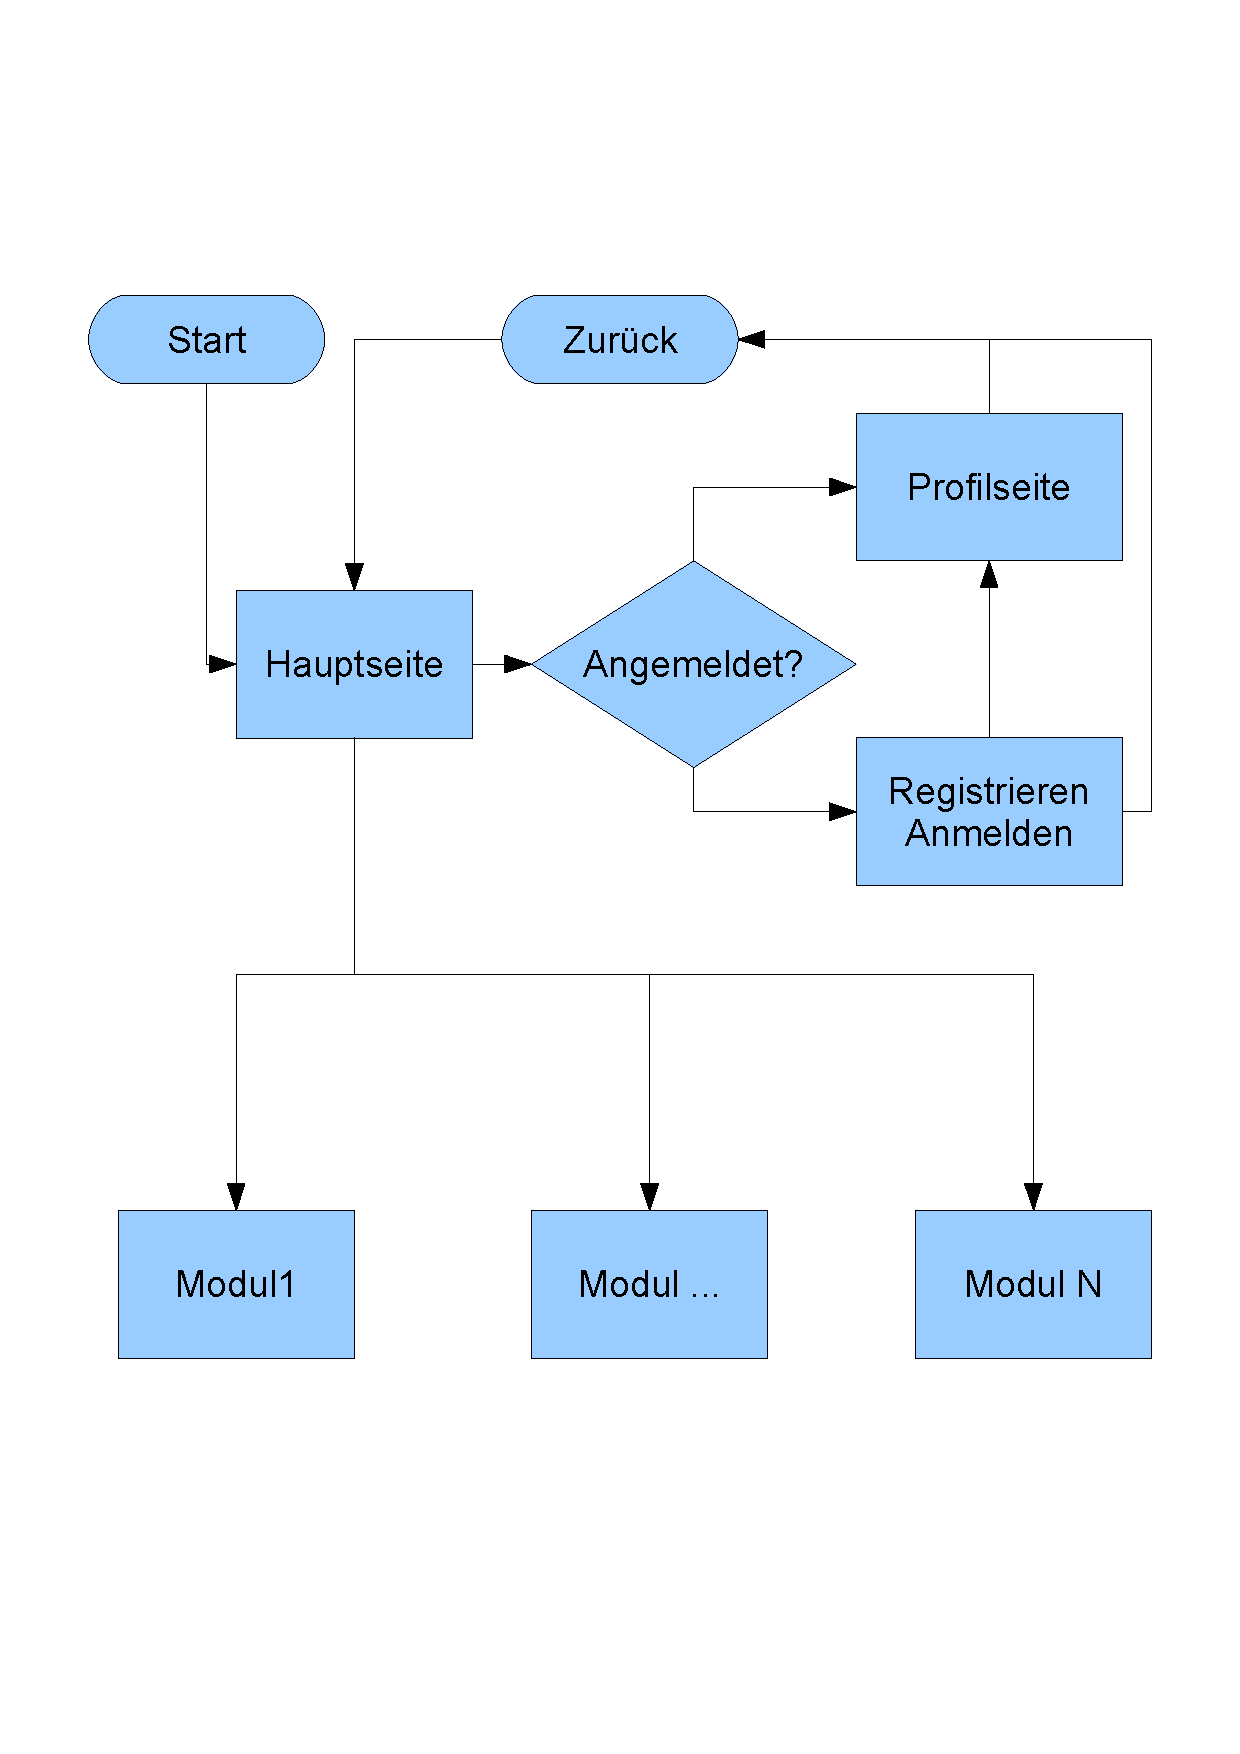
\includepdf[pages=-]{Struktur.pdf}

	\section{Modul-Drehbuch}
	\subsection{Vokabeltrainer}

\modulhauptseite{Vokabeltrainer - Englisch}
\begin{textbereich}
Ich bin ein beschreibender Text :)
\end{textbereich}
\begin{statistikbereich}
hmmm ... ka, was hier so reinkommt ...
\end{statistikbereich}

\modullernseite{Vokabeltrainer - Englisch}{bla}
\begin{navigation}
	\navitem{bla}
\end{navigation}
\begin{inhaltsbereich}
inhalt und so...
\end{inhaltsbereich}

\modultestseite{Vokabeltrainer - Englisch}{bla}
\begin{navigation}
	\navitem{bla}
\end{navigation}
\begin{aufgabenbereich}
aufgaben und so
\end{aufgabenbereich}





\end{document}
